\documentclass{article}[11pt]
\textheight 8.5in
\usepackage{graphicx}
\usepackage{float}%for forcing position of figs
\usepackage{hyperref}
\usepackage{url}
\usepackage{comment}
\usepackage{amsmath}
\usepackage{amssymb}
\usepackage{bm}
\usepackage[makeroom]{cancel}
%%%%%%%%%%%%%%%%%%%%%%%%%%%%%%%%%%%%%%%%%%%%%%%%%%%%%%%%%%%%%%%%%%%%%%%%%%%%%%%%
% based on defs.tex by S. Boyd
% modified by Jie Fu
\newif\ifuseboldmathops
\newif\ifuseittextabbrevs
\useboldmathopstrue   % comment out to use mathbb
%\useittextabbrevstrue % comment out to use non-italic text abbrevs like e.g.
%%%%%%%%%%%%%%%%%%%%%%%%%%%%%%%%%%%%%%%%%%%%%%%%%%%%%%%%%%%%%%%%%%%%%%%%%%%%%%%%

% text abbrevs
\ifuseittextabbrevs
	\newcommand{\cf}{{\it cf.}}
	\newcommand{\eg}{{\it e.g.}}
	\newcommand{\ie}{{\it i.e.}}
	\newcommand{\etc}{{\it etc.}}
	\newcommand{\etal}{{et~al.}}
\else
	\newcommand{\eg}{e.g.}
	\newcommand{\ie}{i.e.}
	\newcommand{\etc}{etc.}
	\newcommand{\etal}{et~al.}
\fi

% standard math sets
\ifuseboldmathops
	%\newcommand{\reals}{{\mbox{\bf R}}}
	\newcommand{\reals}{\mathbf{R}}
	\newcommand{\integers}{\mathbf{Z}}
	\newcommand{\complex}{\mathbf{C}}
	\newcommand{\symm}{\mathbf{S}}  % symmetric matrices
\else
	\newcommand{\reals}{\mathbb{R}}
	\newcommand{\integers}{\mathbb{Z}}
	\newcommand{\complex}{\mathbb{C}}
	\newcommand{\symm}{\mathbb{S}}  % symmetric matrices
\fi

% control theory sets
\ifuseboldmathops
	\newcommand{\HH}{\mathbf{H}}
	\newcommand{\LL}{\mathbf{L}}
\else
	\newcommand{\HH}{\mathbb{H}}
	\newcommand{\LL}{\mathbb{L}}
\fi

% probability operators
\ifuseboldmathops
	\newcommand{\Expect}{\mathop{\bf E{}}\nolimits}
	\newcommand{\Prob}{\mathop{\bf P{}}\nolimits}
\else
	\newcommand{\Expect}{\mathop{\mathbb{E}{}}\nolimits}
	\newcommand{\Prob}{\mathop{\mathbb{P}{}}\nolimits}
\fi

% convex operators
\ifuseboldmathops
	\renewcommand{\Re}{\mathop{\bf Re}}
	\renewcommand{\Im}{\mathop{\bf Im}}
	
	\newcommand{\prox}{\mathop{\bf prox}} % proximal operator
	\newcommand{\dom}{\mathop{\bf dom}}   % domain
	\newcommand{\aff}{\mathop{\bf aff}}   % affine hull
	\newcommand{\cl}{\mathop{\bf cl}}     % closure
	\newcommand{\intr}{\mathop{\bf int}}  % interior
	\newcommand{\Co}{\mathop{\bf Co}}     % convex hull
	\newcommand{\relint}{\mathop{\bf rel int}} % relative interior
	\newcommand{\bd}{\mathop{\bf bd}}     % boundary
	
	\newcommand{\Tr}{\mathop{\bf Tr}}
	\newcommand{\diag}{\mathop{\bf diag}}
\else
	\renewcommand{\Re}{\mathop{\mathrm{Re}}}
	\renewcommand{\Im}{\mathop{\mathrm{Im}}}
	
	\newcommand{\prox}{\mathop{\mathrm{prox}}} % proximal operator
	\newcommand{\dom}{\mathop{\mathrm{dom}}}   % domain
	\newcommand{\aff}{\mathop{\mathrm{aff}}}   % affine hull
	\newcommand{\cl}{\mathop{\mathrm{cl}}}     % closure
	\newcommand{\intr}{\mathop{\mathrm{int}}}  % interior
	\newcommand{\Co}{\mathop{\mathrm{Co}}}     % convex hull
	\newcommand{\relint}{\mathop{\mathrm{rel int}}} % relative interior
	\newcommand{\bd}{\mathop{\mathrm{bd}}}     % boundary
	
	\newcommand{\Tr}{\mathop{\mathrm{Tr}}}     % trace
	\newcommand{\diag}{\mathop{\mathrm{diag}}} % diagonal matrix
\fi

% useful non-bold operators
\newcommand{\eqbydef}{\mathrel{\stackrel{\Delta}{=}}}
\newcommand{\eqbyset}{\mathrel{\stackrel{\mathrm{set}}{=}}}
\newcommand{\argmax}{\mathop{\mathrm{argmax}}}
\newcommand{\argmin}{\mathop{\mathrm{argmin}}}

% lin alg stuff
\newcommand{\Span}{\mathop{\mathrm{span}}}
\newcommand{\Range}{\mathop{\mathrm{range}}}
\newcommand{\Null}{\mathop{\mathrm{null}}}
\newcommand{\rank}{\mathop{\mathrm{rank}}}

\newcommand{\ones}{\mathbf 1}
\newcommand{\lambdamax}{{\lambda_{\rm max}}}
\newcommand{\lambdamin}{{\lambda_{\rm min}}}
\newcommand{\sigmamax}{{\sigma_{\rm max}}}
\newcommand{\sigmamin}{{\sigma_{\rm min}}}

% newcommend for IRL


\newcommand{\supp}{\mathsf{supp}}
\newcommand{\soft}{\mathsf{soft}}
\newcommand{\abs}[1]{\lvert#1 \rvert}
\newcommand{\norm}[1]{\lVert#1 \rVert}
\usepackage{acronym}

\newcommand{\terminal}{\mathsf{terminal}}
\acrodef{mdp}[MDP]{Markov Decision Process}
\newcommand{\expect}{\mathbb{E}}
\newcommand{\normal}{\mathcal{N}}


\newcommand{\todo}[1]{\textcolor{red}{#1}}
\newtheorem{assumption}{Assumption}
\newtheorem{claim}{Claim}
\newtheorem{definition}{Definition}

\newcommand{\Lagrange}{\mathcal{L}}

\newcommand{\Always}{\Box \, }
\newcommand{\Eventually}{\Diamond \, }
\newcommand{\Next}{\bigcirc \, }
\newcommand{\sink}{\mathsf{sink} }

%\newcommand{\Next}{\kern0.5ex\vcenter{\hbox{$\scriptstyle\bigcirc$}}\kern0.5ex}
\newcommand{\Until}{\mbox{$\, {\sf U}\,$}}
\newcommand{\WeakUntil}{\mbox{$\, {\sf W}\,$}}
\newcommand{\BoolTrue}{\mbox{\sf true}}
\newcommand{\BoolFalse}{\mbox{\sf false}}
\newcommand{\calA}{\mathcal{A}}
\newcommand{\calAP}{\mathcal{AP}}
\newcommand{\calW}{\mathcal{W}}

\acrodef{mcmc}[mcmc]{Monte Carlo Markov chain}
\begin{document}
\begin{center}
\textbf{ \Large Learning MDP with second-hand samples}
\\
Siddharthan Rajasekaran, 
Jie Fu\\
 sperundurairajas@wpi.edu,
 jfu2@wpi.edu
\end{center}

\section{Summary of Discussions}
In this report, we are interested in reducing the sample complexity of
PAC-learning in MDP using similarity between different
states. Our approach is to integrate Expectation-Maximization with
PAC-learning.


\section{Problem statement}
We consider an MDP $(S,A, P, r)$ in which the transition probability
function $P$ is unknown. Moreover, the state space can be partitioned
into different clusters $\bigcup_{i=1}^m \Pi_i=S$. The system dynamics
in each cluster is homogeneuous. The class of each state is only
observed through uncertain sensors. For example, in Mars rover
exploration task, the system can only tell from images a probabilistic
distribution of the types of the ground: At state $s$, the probability
that the current state is in type ``sand'' is $0.7$ and in type
``gravel'' is $0.2$. This information provided by the sensor is
considered \emph{side information} for the system. 

Problem: Given the side information, develop an algorithm that learns
the underlying transitio function $P$ from data collected through
exploring the state space.


Notation: Let the set of classes be $\mathcal{C} = \{1,\ldots,m\}$. Given a
state $s\in S$, if it is in class $j$, the transition function
$P(s,a) = \Psi_j(s,a)$ where
$\Psi_j :S\times A\times S\rightarrow[0,1]$ is the transition function
given that all states in the MDP is in class $j$.

\emph{Data set}: The data set is a sequence of tuples
$D =  \{(s_i, a_i, s_{i+1}, p_i),i=1,\ldots, N\}$ where
$(s_i,a_i, s_{i+1})$ is an observed transition at step $i$ and
$p_i: \mathcal{C} \rightarrow [0,1]$ is a probability distribution
over the classes. $p_i(j)$ is the probability that the state $s_i$
belongs to class $j$. 

\begin{assumption}
\label{assumelinear}
Using conditional probability, for any $s\in S$, we have
\[
  P(s' \mid s,a) = \sum_{j=1}^m  P(s' \mid s,a , c_j) p(c_j \mid s)  = \sum_{j=1}^m \Psi_j(s'\mid s,a ) p(c_j\mid s).
\]
\end{assumption}
 
\emph{Problem 1:} Assuming ~\ref{assumelinear} Given the data $D$,
compute the transition functions $\{\Psi_j \mid j=1,\ldots, m\}$ as
well as the bounds of error confidence intervals.

\emph{Problem 2:} In the second case, we consider that the state space
of the MDP is not clearly partitioned into $m$ different
classes. Rather, a state with $0.5$ ``sand'' and $0.5$ ``gravel''
could be a mixture of ground condition that is neither sand or gravel,
but some type in between.  Now, the conditional probability cannot be
used directly and the relation between $P(s'\mid s,a)$ and
$\Psi_j(s'\mid s,a )$ may no longer be linear. 

\subsection{When the assumption holds}
We consider systems which evolve at discrete instances of time. The
time index can be $1,2,\ldots, N$ where $N$ can be finite.  Let
$\cal T$ be an index set, which can be finite or countably
infinite. Assume also that there is an underlying probability space
$(\Omega, S, P)$ with respect to which all random variables are
defined. A family of random variables $w_k$, $k\in \cal T$ is a
discrete time stochastic process which is the noise to the system. The
stochastic system
\[
x_{k+1}   =f(x_k, u_k, w_k), \quad k=0,1,\ldots.
\]
where $x_k \in X$ and $u_k\in U$ are state and input at time step $k$.


% An \ac{mdp} can be obtained from discretization of the state and input
% spaces. Let the discretized state space be $S=\{s_1,\ldots, s_n\}$ and
% discretized input be $A = \{a_1,\ldots, a_p\}$.

% Given $x\in X$ and $u \in U$, the probability transition function
% $P(x' \mid x, u )= p(w)\cdot 1_{x' = f(x,u, w)}$. Denote $[x]$ be the
% discrete state in the MDP which contains $x$, we have 
% \[
% P([x'] \mid [x], u) = \int_{z\in [x]} \int_w  1_{f(z,u, w)\in [x']} dw
% \]

Now, consider the case with different classes, it is similar to the
case that the system dynamics has a hidden parameter variable
$\theta_k$ and evolve according to
\[
x_{k+1} =f (x_k, u_k, \theta_k , w_k), \quad k=0,1,\ldots,
\]
where $\theta_k$ is the parameter when the system and takes discrete
values in $\{\theta_j, j=1,\ldots, m\}$. As an example of $\theta_k$,
in Mars rover case, $\theta_k$ can be the friction coefficient with
respect to the ground. The domain $\Theta$ of friction parameter can
be continuous. In this case, the different classes may be considered
as a finite subset of the parameter space $\Theta$. Particular, if we
assume $\Theta$ is a probability simplex, then $\theta_j$ can be
picked to be affinely independent points that determine the simplex
$\Theta$.

Consider any $\theta =\sum_{j} v_j \theta_j$ with $\sum_{j}v_j=1$, for
any state action pair $(x,a)$ and a noise $w$, the next state is
\[
x '  = f(x,a,\theta, w)  = f(x,a ,\sum_{j} v_j \theta_j,w  ) 
\]

\begin{claim}
  In the case we can represent the vector field
  $f(x,u,\theta, w)= g_1(x,u)^T\theta + g_2(x,u,w)$, then 
\[
x' = f(x,a,\theta, w) =\sum_{j} v_j f(x,a,\theta_j, w)
\]
where $\theta =\sum_{j} v_j \theta_j$ holds.
\end{claim}
Proof: \begin{align*}
x_{k+1}  = & g_1(x,u)^T  \theta + g_2(x,u,w)\\
 = & \sum_{j} v_j g_1(x,u)^T \theta_j + g_2(x,u,w)  \\
= & \sum_j  v_j g_1(x,u)^T \theta_j + \sum_j v_j g_2(x,u,w)  \\
=  &\sum_j v_j (g_1(x,u)^T\theta_j + g_2(x,u,w)) = \sum_j v_j  f(x,a,\theta_j, w)
\end{align*}
since $\sum_j v_j =1$.

It is as if we allow the system evolves independently in $m$ different
systems parameterized by different $\theta_j$ and the combine the
output in these systems given the weight $v_j$. 




\section{Problem 1: Learning with side information}
% The paradigm of PAC-learning is to recover a
% near-optimal policy with high confidence using data collected from
% this MDP. However, a big limitation in PAC is that the sampling
% complexity. We aim to reduce the sample complexity by reusing samples
% collected from one state to another state which is similar (in the
% probability transition function).

% A simpler problem: Let's assume the state $S$ can be partitioned into
% a set of disjoint sets $\{c_1,c_2,\ldots, c_n\}$ for some $n\ge 0 $,
% which is unknown to us. The best way to reuse sample is that for any
% $i$, for each $s,t\in S_i$ the samples collected from $s$ and $t$ will
% be used to determine the same probability transition function for the
% partition $c_i$.


% \section{A simple analysis on the weight}
% A simpler question is, if two states are known to be similar, what is
% the meaning of weights? For now, let's consider a known MDP. Let
% $S = \{1,\ldots, N\}$ be the indexed state set. We have two states
% $s_1,s_2$. We only have samples from $s_1$, which is a set of observed
% state-action-nextstate tuples
% $Y_1 =\{(s_1,a', s'), a' =a_1,a_2,\ldots, a_N, s' = s_1',s_2' ,\ldots,
% s_N'\}$.
% With some transformtion of the state space, we can assume the set of
% all possible resulting states from $s_1$ and $s_2$ are the same for
% the same action. So, the question is, if this set of actions
% $a_1,a_2,\ldots,a_N$ were taken from state $s_2$, what will be our
% sampled data $Y_2$?

% Given an action $a$ enabled from both $s_1$ and $s_2$, let's assume
% for now that we know the transition probability
% $P_1 = [P(s_1,a,s')]_{s' \in S}$ and $P_2 = [P(s_2,a,s')]_{s' \in
%   S}$.

% We denote $count_1[t]$ the counts of transition $(s,a,t)$ in the
% sample $Y_1$. $count_1$ a
% data sample set generated i.i.d. from a sample distribution $P_1$, but
% we are interested in estimating the expected value of the samples for
% transition $(s_2, a, t)$, that is $count_2[t] = \mathbb{E}_{P_2}[\sum_{a_i=a} (s_2,a_i,t)]$, under a
% different distribution $P_2$, without directly sampling $P_2$.

% This problem is importance sampling.  In importance sampling, this is
% achieved by averaging the samples weighted by the ratio of their
% likelihood $\rho_t = \frac{P_2(t)}{P_1(t)}$. That is, $count_2$ is
% estimated as:
% \begin{equation}
% \label{weight}
% count_2[t] = {\rho_t count_1[t]}
% \end{equation}
% Because $count_1[t] /\sum_{s'} count_1[s'] \approx P_1(t)$ and
% $count_2[t] /\sum_{s'} count_2[s'] \approx P_2(t)$, let's assume that
% the total number of samples generated from two distribution is the
% same, i.e., $ \sum_{s'} count_1[s'] =\sum_{s'} count_2[s']$, then it
% is clear that
% \[
% count_1[t]/count_2[t] \approx P_1(t)/P_2(t).
% \]
% which is equivalent to \eqref{weight}.

% Thus, obtaining a sample $count_1[t]$ from $s_1$ is equivalent to that
% obtaining  a sample $count_2[t]$ from $s_2$ which is $count_2[t]  =
% count_1[t] \rho_t$. 

% \emph{Correct weight}: $P_2(t)/P_1(t)$.

% \emph{Accurate side information}: If we do not know $P_1$ and $P_2$
% but known $\rho_t$ for any next state $t$, then we are good to
% perform weighted reusing of samples. %  \section{Bibliography}

In the following sections, we will see two different ways of finding the transition probability for each terrain given a trajectory sampled from the real system with time varying probability distribution over the terrains. In both the methods we will aggregate homeomorphic states and actions. For example, facing North and taking the action ``East" is same as facing East and taking the action ``South". Hence the state action pairs (North, East) = (East, South). 
%%
\subsection{EM with PAC}
In this section, we will first see why, given a sequence of events sampled from a probability distribution over several events, the probability of a particular event is given by $P(event) = \frac{\# event}{\# all \ events}$, where $\#$ denotes the total number of times an event occurred in the sample. This informs us about how the problem of interest can be formulated similarly. 

Consider the case of learning $T(s'|s,a)$ in an MDP with just one terrain given a trajectory $\tau = [s_1,a_1,s_2,a_2, ..., s_T,a_T]$. Let the current estimate of $T(s'|s,a)$ be $\Psi(s'|s,a)$ 

The probability of sampling the above trajectory given $\Psi$ and the control actions $\textbf{a} = [a_1, a_2, ..., a_T]$ is given by

\begin{equation}
P(\tau|\Psi || a) = \prod_t \Psi(s_{t+1}|s_t,a_t)
\end{equation} where $||$ indicates conditioning over variables we do not have control over for our problem of estimating $\Psi$. The log likelihood of the trajectory is given by $\mathcal{L} = \ln \Big[ \prod_t \Psi(s_{t+1}|s_t,a_t) \Big]$. The maximum likelihood solution over $\Psi$ for the problem can be formulated as, 

\begin{align}
\label{ori_objective}
\Psi^* = \arg \max_\Psi  \sum_t \ln \Psi(s_{t+1}|s_t,a_t)\\
\text{s.t. }\sum_{s'} \Psi(s'|s,a) = 1, \forall s,a
\end{align}The Lagrangian is given by, 

\begin{align}
\label{Lagrangian}
L &= \sum_t \ln \Psi(s_{t+1}|s_t,a_t)  + \sum_{s,a} \lambda_{s,a} \Big[ \sum_{s'} \Psi(s'|s,a) - 1\Big]\\
\nabla_{\Psi(s'|s_{t_0},a_{t_0})}L &= \sum_{t:s_{t+1} = s', s_t = s_{t_0}, a_t = a_{t_0}} \frac{1}{\Psi(s_{t+1}|s_t,a_t)} + \lambda_{s_{t_0},a_{t_0}} = 0\\
\label{prop}
(or) \ \ \  \Psi(s_{t+1}|s_t,a_t) &\propto \sum_{t:s_{t+1} = s', s_t = s_{t_0}, a_t = a_{t_0}}1\\
\label{ML_oridinary_case}
\implies \ \ \Psi(s'|s_{t_0},a_{t_0}) &= \frac{\#(s_{t_0},a_{t_0},s')}{\#(s_{t_0},a_{t_0})}
\end{align}

The above formula Eq. \ref{ML_oridinary_case} is the result of maximum likelihood estimate of the underlying probability distribution $\Psi$. In our problem, we also have another variable namely the type of environment. This can be treated as a hidden class variable in case of clustering and we can use Expectation (over the type environment) - Maximization (similar to the maximization in Eq. \ref{Lagrangian}). Since we know the distribution over class, $P(c|t)$, at time $t$  from the observations, we marginalize out time to get $P(c_j|s_t,a_t,s_{t+1})$. The maximization problem can be written as,
 \begin{align}
\Psi^* &= \arg \max_{\Psi_{c_1} ... \Psi_{c_m}} \sum_t \ln P(s_{t+1}|s_t,a_t,\Psi_{c_1} ... \Psi_{c_m})\\
\label{em_ification}
&=\arg \max_{\Psi_{c_1} ... \Psi_{c_m}} \sum_{t=1}^T\sum_{j=1}^m P(c_j|s_t,a_t,s_{t+1},\Psi_{c_1} ... \Psi_{c_m})\ln P(s_{t+1}, c_j|s_t,a_t,\Psi_{c_1} ... \Psi_{c_m})\\
&=\arg \max_{\Psi_{c_1} ... \Psi_{c_m}} \sum_{t=1}^T\sum_{j=1}^m \Big[\sum_{t'}\big[P(c_j|t')P(t'|s_t,a_t,s_{t+1})\big]\ln P(s_{t+1}, c_j|s_t,a_t,\Psi_{c_1} ... \Psi_{c_m})\Big]\\
&=\arg \max_{\Psi_{c_1} ... \Psi_{c_m}} \sum_{t=1}^T\sum_{j=1}^m\Big[ \underbrace{\sum_{t':(s_{t'},a_{t'},s_{t'+1}) = (s_t,a_t,s_{t+1})}\Bigg[\frac{P(c_j|t')}{\#(s_t,a_t,s_{t+1})}\Bigg]}_{\beta_{tj}}\ln P(s_{t+1}, c_j|s_t,a_t,\Psi_{c_1} ... \Psi_{c_m})\Big]
 \end{align} where we get Eq. \ref{em_ification} from EM.  We know the value of $P(c_j|t)$ from the sensor, hence we replace the inner sum by $\beta_{tj}$ which denotes the probability of class $c_j$ given the tuple $(s_t,a_t,s_{t+1})$. That is, 
 
 
\begin{align}
\Psi^* &= \arg \max_{\Psi} \sum_{t=1}^T\sum_{j=1}^m \beta_{tj} \ln P(s_{t+1}, c_j|s_t,a_t,\Psi_{c_1} ... \Psi_{c_m})\\
 &= \arg \max_{\Psi} \sum_{t=1}^T\sum_{j=1}^m \beta_{tj} \ln \big[P(s_{t+1}|c_j, s_t,a_t,\Psi_{c_1} ... \Psi_{c_m})P(c_j|s_t,a_t)\big]\\
 \label{simplified_conditionals}
  &= \arg \max_{\Psi} \sum_{t=1}^T\sum_{j=1}^m \beta_{tj} \ln \Psi_{c_j}(s_{t+1}| s_t,a_t) + \underbrace{\ln P(c_j|s_t,a_t)}_{\text{const.}}\\
  \label{em_objective_full}
   \Psi^*   &=  \sum_{j=1}^m \arg \max_{\Psi_{c_j}}\sum_{t=1}^T\beta_{tj} \ln \Psi_{c_j}(s_{t+1}| s_t,a_t) \\
  \label{em_objective}
 \Psi^*_{c_j}   &=  \arg \max_{\Psi_{c_j}}\sum_{t=1}^T\beta_{tj} \ln \Psi_{c_j}(s_{t+1}| s_t,a_t) \\
 &\text{s.t. } \sum_{s'} \Psi_{c_j}(s'|s,a) = 1, \forall s,a
\end{align} We get Eq. \ref{simplified_conditionals} from the fact that the class variable $c_j$ just picks the corresponding probability distribution $\Psi_{c_j}$. We get Eq. \ref{em_objective} since each term in the summation is independent of other terms in the maximization problem. The objective in Eq. \ref{em_objective} is similar to Eq. \ref{ori_objective} except that each term is multiplied by $\beta_{tj}$. Hence, by following the same steps we get (similar to Eq. \ref{prop}), 

\begin{align}
\Psi_{c_j}(s'|s_{t_0}, a_{t_0}) &\propto \sum_{t:(s_{t},a_{t},s_{t+1}) = (s_{t_0},a_{t_0},s')}\beta_{tj}\\
& \propto \beta_{tj} \sum_{t:(s_{t},a_{t},s_{t+1}) = (s_{t_0},a_{t_0},s')} 1\\
& \propto \frac{\sum_{t':(s_{t'},a_{t'},s_{t'+1}) = (s_{t_0},a_{t_0},s')}P(c_j|t')}{\cancel{\#(s_t,a_t,s_{t+1})}} \cdot \cancel{\#(s_t,a_t,s_{t+1})}\\
\Psi_{c_j}(s'|s_{t_0}, a_{t_0}) &= \frac{\sum_{t':(s_{t'},a_{t'},s_{t'+1}) = (s_{t_0},a_{t_0},s')}P(c_j|t')}{\sum_{t':(s_{t'},a_{t'}) = (s_{t_0}, a_{t_0})}P(c_j|t')}\\
&= \frac{\text{effective}\#(s_{t_0},a_{t_0},s')}{\text{effective}\#(s_{t_0},a_{t_0})}
\end{align}
 
\subsection{Marginalization with PAC}
Consider a sample trajectory $\tau$ generated with an arbitrary distribution over classes. The maximum likelihood probability of observing a tuple $(s_{t_0},a_{t_0}, s')$ under the time varying class distribution is given by 
\begin{align*}
P(s'|s_{t_0},a_{t_0}) &= \frac{\#(s_{t_0},a_{t_0}, s')}{\#(s_{t_0},a_{t_0})}
\end{align*}We can rewrite $P(s'|s_{t_0},a_{t_0})$ by marginalizing the class variable $c_j$ as
\begin{align*}
P(s'|s_{t_0},a_{t_0}) &= \sum_{j=0}^mP(s',c_j|s_{t_0},a_{t_0})\\
&= \sum_{j=0}^mP(s'|c_j,s_{t_0},a_{t_0})P(c_j|s_{t_0},a_{t_0})\\
&= \sum_{j=0}^mP(s'|c_j,s_{t_0},a_{t_0})\sum_tP(c_j|t)P(t|s_{t_0},a_{t_0})\\
&= \sum_{j=0}^mP(s'|c_j,s_{t_0},a_{t_0})\sum_{t:(s_{t},a_{t}) = (s_{t_0},a_{t_0})}\frac{P(c_j|t)}{\#(s_{t_0},a_{t_0})}\\
&= \sum_{j=0}^m \Psi^*_{c_j}(s'|s_{t_0},a_{t_0})\sum_{t:(s_{t},a_{t}) = (s_{t_0},a_{t_0})}\frac{P(c_j|t)}{\#(s_{t_0},a_{t_0})}\\
\text{Let } \ \alpha_{tj} &= \sum_{t':(s_{t'},a_{t'}) = (s_{t},a_{t})} \frac{P(c_j|t')}{\#(s_{t},a_{t})}\\
%TODO: Change alpha_t to the correct subscript t
\therefore \frac{\#(s_{t_0},a_{t_0}, s')}{\#(s_{t_0},a_{t_0})} & = \sum_{j=0}^m \Psi^*_{c_j}(s'|s_{t_0},a_{t_0})\alpha_{tj}\\
&= [\alpha_{t1}, \alpha_{t2} \hdots \alpha_{tm}] \begin{bmatrix}
\Psi^*_{c_1}\\\Psi^*_{c_2}\\ \vdots\\ \Psi^*_{c_m}
\end{bmatrix}\\
&= \bm{\alpha}_t^T \begin{bmatrix}
\Psi^*_{c_1}\\\Psi^*_{c_2}\\ \vdots\\ \Psi^*_{c_m}
\end{bmatrix}
\end{align*}

The above equation has $m$ unknowns $(\Psi^*_{c_j}, \forall j)$. We can however, solve the above equation by segmenting the existing trajectory into $m$ pieces. We will denote the piece index in the super script like $\bm{\alpha}_t^{T(j)}$. 


\begin{align*}
\text{Let }A &= \begin{bmatrix}
\bm{\alpha}_t^{T(1)}\\ \bm{\alpha}_t^{T(2)}\\ \vdots\\ \bm{\alpha}_t^{T(m)}
\end{bmatrix}\\
\begin{bmatrix}
P^{(1)}\\ P^{(2)}\\ \vdots\\ P^{(m)}
\end{bmatrix} &= A \begin{bmatrix}
\Psi^*_{c_1}\\\Psi^*_{c_2}\\ \vdots\\ \Psi^*_{c_m}
\end{bmatrix}\\
\therefore \begin{bmatrix}
\Psi^*_{c_1}\\\Psi^*_{c_2}\\ \vdots\\ \Psi^*_{c_m}
\end{bmatrix} &= A^{-1}\begin{bmatrix}
P^{(1)}\\ P^{(2)}\\ \vdots\\ P^{(m)}
\end{bmatrix}
\end{align*} where $P^{(j)}$ is $P^{(j)}(s'|s_{t_0},a_{t_0})$ and $\Psi_{c_j}$ is $\Psi_{c_j}(s'|s_{t_0},a_{t_0})$. We solve the above system of equations for all possible combinations of $(s_{t_0},a_{t_0},s')$ that occur in the trajectory $\tau$. 

Note that we need to be exposed to atleast $m$ different distributions
over the terrains for the matrix $A$ to be non singular. The same is
actually necessary even in case of the EM formulation to meaningfully
estimate the underlying distributions. In case we have a trajectory
with only one distribution over the terrain for all $t$, the EM sets
$\Psi^*_{c_1} = \Psi^*_{c_2} ... = \Psi^*_{c_m}$ (which is in fact the
maximum likelihood solution).

\subsection{Results}

We tested the marginalization based method on a toy example with four states and two classes. Each state has two actions $0$ and $1$. In the first class $c_1$, given the current state $s_t$, the action $0$ results in a uniform distribution over the next possible states $s_{t+1}$ while that of action $1$ results in a Gaussian centered at the current state. The second class just reverses the effects of actions $0$ and $1$. That is, action $1$ results in a uniform distribution and, action $0$, in a Gaussian.

We generate a trajectory using the above conditions and use it to learn the underlying transition matrix of each class. We assume that the probability of class $c_1$ changes from $0.05$ to $0.95$ linearly along the trajectory and that of $c_2$ is just $1 - P(c_1)$. We split the trajectory into two halves since the first and the second has a different average class distributions. 


The following graph shows how the norm of the error matrix (difference of learned and the underlying transition matrices) falls with increasing length of the trajectory. 

\begin{figure}[H]
\centering
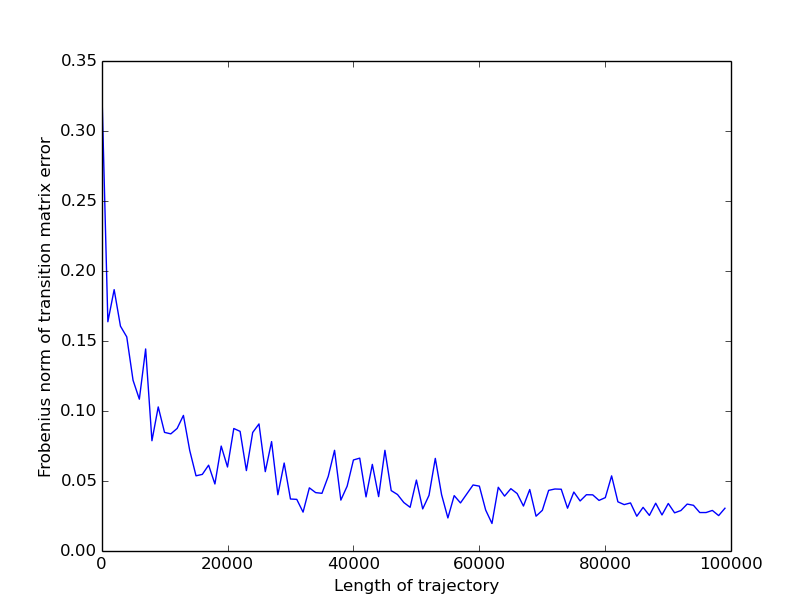
\includegraphics[width=1.2\linewidth]{images/error_vs_l}
\caption{Norm of error between the learned transition matrix and the ground truth vs the length of the trajectory.}
\end{figure}

% \begin{comment}
% We consider the case when the states of the MDP can be classified into
% $N$ different clusters. At the same time, there is additional side
% information helps us to classify the state. The side information is
% given for each state $s$, $p(s,j)$ is the probability of state $s$
% being in cluster $j$, and $\sum_{j=1}^N p(s,j)=1$.

% Assumption: For any state in one cluster, the probabilistic
% transition function follows the same distribution $P(i,a)$, for any
% $a\in A$.  

% Now, suppose for state $s$ we have obtained sampled transitions
% $count(s,a,t)$, and the side information is given by
% $p(s)\in \mathcal{D}(\mathcal{C})$. We aim to solve, how many
% equivalent samples shall we use for each cluster?

% $count(s,a,t) \approx \sum_{i=1}^N p(s,i) P(s,a,t \mid s\in C_i) count(s,a)$
% where $P(s,a,t\mid s\in C_i ) \approx
% \frac{count_i(s,a,t)}{count(s,a)}$.

% If we substitute into the equation, it becomes 
% \[
% count(s,a,t) \approx \sum_{i=1}^N p(s,i)
% \frac{count_i(s,a,t)}{count(s,a)}count(s,a) = \sum_{i=1}^N p(s,i)
% \frac{count_i(s,a,t)}.
% \]

% There is no unique solution to this equation because the number of
% unknowns is $N>1$. However, if we collect from $N $ times the count
% from the same  state $s$, then we have $N$ different equations
% \[
% count^k(s, a,t) \approx \sum_{i=1}^N p(s,i)
% count_i(s,a,t).
% \]
%
% \end{comment}
% \bibliographystyle{plain}
% \bibliography{bibfile}
\end{document}
